\documentclass[11pt,a4paper]{article}

\usepackage[margin=1in]{geometry}
\usepackage{amsmath,amssymb,amsthm}
\usepackage{graphicx}
\usepackage{booktabs}
\usepackage{siunitx}
\usepackage{hyperref}
\usepackage{xcolor}
\usepackage[numbers,sort&compress]{natbib}
\usepackage{tikz}
\usetikzlibrary{arrows.meta,positioning}
\usepackage{caption}
\usepackage{array}

\hypersetup{colorlinks=true,linkcolor=blue!50!black,citecolor=blue!50!black,urlcolor=blue!50!black}
\sisetup{detect-all,per-mode=symbol}
\newcommand{\hyp}[1]{\textcolor{blue!45!black}{\textsf{\small #1}}}

\title{\textbf{A Storage-Ring Steady-State-Microbunching Undulator Architecture\\
for a High-Average-Power \SI{13.5}{\nano\meter} Lithography Source}\\[4pt]
\large Architecture~I of the lumen EUV source family (rank~2); shared experimental gate with the
compact SSMB-Compton architecture}

\author{lumen verified-hypothesis lab \\ \texttt{dancinlab/lumen}}
\date{Draft, as-of 2026-06}

\begin{document}
\maketitle

\begin{abstract}
We specify the \emph{storage-ring steady-state-microbunching (SSMB) undulator} architecture for a
continuous-wave, coherent \SI{13.5}{\nano\meter} EUV source at the $\sim$\SI{100}{\watt}-class
average power high-volume lithography requires. A several-hundred-MeV electron beam stored in a ring
is microbunched at the radiation wavelength every turn, so $N$ electrons radiate \emph{coherently}
($P\!\propto\!N^{2}$, a $\sim\!10^{6}\times$ enhancement) and, because the ring reuses the beam, the
power is delivered continuous-wave rather than in the dumped single-shot of a single-pass
free-electron laser (FEL). This is the missing middle between the incumbent laser-produced plasma and
the funded conventional energy-recovery-linac FEL: coherent average power without a dumped beam.
The mechanism is proof-of-principle demonstrated~\citep{deng2021}; \SI{13.5}{\nano\meter} kilowatt
operation is undemonstrated. We give the closed-form architecture, its subsystems, and its binding
gate --- steady-state microbunching at \SI{13.5}{\nano\meter} precision --- which it \emph{shares}
with the compact SSMB-Compton architecture (companion paper~II): one experiment de-risks both. The
analysis is closed-form and reference-matched; it claims convergence on the same physics, not
precedence.
\end{abstract}

\section{Introduction}
This is Architecture~I of the lumen EUV source family. For the EUV-litho high-flux requirement the
family ranks eight source classes; this paper specifies rank~2, the SSMB undulator. It is one of two
\emph{novel} architectures (the other, rank~3, is the compact SSMB-Compton source of the companion
paper). The two are genuinely different machines --- different beam energy ($\sim$\SI{511}{\mega\electronvolt}
vs.\ \SI{7}{\mega\electronvolt}), different radiation mechanism (undulator vs.\ inverse-Compton),
different footprint --- so we document them separately, while making explicit that they reduce to one
shared experimental gate (Section~\ref{sec:gate}).

\section{Background: the wall is flux, not wavelength}
An undulator of period $\lambda_u$ radiates at $\lambda=(\lambda_u/2\gamma^{2})(1+K^{2}/2)$, so
wavelength is an electron-energy dial with no physical floor (\hyp{H\_011}). The binding limit for an
FEL is beam slice energy spread: gain collapses once $\sigma_\delta/\rho\gtrsim1$~\citep{mingxie},
and a representative \SI{0.5}{\percent} laser-plasma beam sits $\sim\!5\times$ over budget, never
lasing at \SI{13.5}{\nano\meter} (\hyp{H\_031}; demonstrated LPA-FEL floor $\sim$\SI{25}{\nano\meter}
\citep{xiao2026}). A conventional RF-compressed beam clears this (FLASH lased \SI{13}{\nano\meter},
2006), which is why the funded near-term answer is a shared conventional ERL FEL (\hyp{H\_030}). The
architecture here makes flux --- average power --- the operative wall, and breaks it by coherence.

\section{Architecture}
\label{sec:arch}
\begin{figure}[t]
\centering
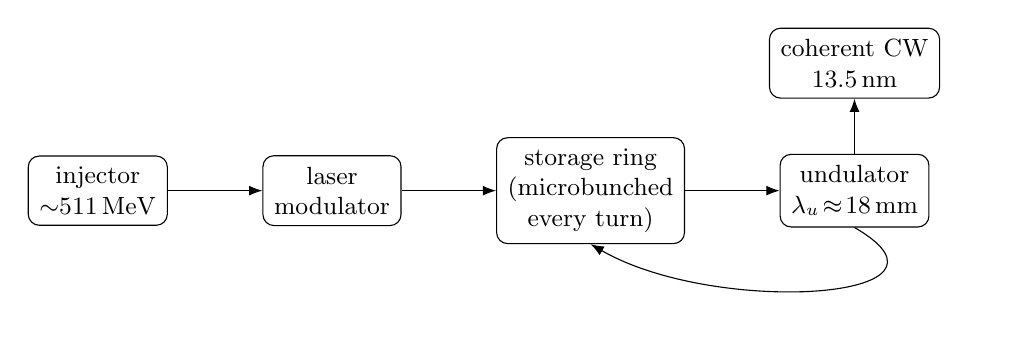
\begin{tikzpicture}[node distance=7mm and 12mm,every node/.style={font=\small},
  box/.style={draw,rounded corners,align=center,inner sep=4pt,minimum height=8mm}]
  \node[box] (gun) {injector\\$\sim$\SI{511}{\mega\electronvolt}};
  \node[box,right=of gun] (mod) {laser\\modulator};
  \node[box,right=of mod] (ring) {storage ring\\(microbunched\\every turn)};
  \node[box,right=of ring] (und) {undulator\\$\lambda_u\!\approx\!\SI{18}{\milli\meter}$};
  \node[box,above=of und] (out) {coherent CW\\\SI{13.5}{\nano\meter}};
  \draw[-{Latex}] (gun)--(mod); \draw[-{Latex}] (mod)--(ring); \draw[-{Latex}] (ring)--(und);
  \draw[-{Latex}] (und)--(out);
  \draw[-{Latex}] (und.south) to[out=-30,in=-30,looseness=1.4] (ring.south);
\end{tikzpicture}
\caption{SSMB undulator architecture. The stored beam is laser-modulated and microbunched at the
radiation wavelength every turn; on-axis undulator emission is coherent ($P\!\propto\!N^2$) and
continuous-wave because the ring reuses the beam.}
\label{fig:arch}
\end{figure}

In a storage ring $N$ electrons normally radiate incoherently ($P\!\propto\!N$). Microbunched at the
radiation wavelength ($\sigma_z\!\ll\!\lambda$) they radiate coherently ($P\!\propto\!N^{2}$,
$\sim\!10^{6}\times$). \emph{Steady-state} microbunching sustains the bunching every turn, so the
coherent power is continuous-wave from a reused beam (\hyp{H\_043}). The program target is
$\sim$\SI{1}{\kilo\watt} at \SIrange{13}{14}{\nano\meter}~\citep{deng2022}, $\geq\!10\times$ the
$\sim$\SI{100}{\watt} HVM floor (\hyp{H\_005}). Because the radiation is on-axis undulator emission,
this architecture carries \emph{no} Compton bandwidth-collection flux tax; its cost is the higher
beam energy ($\sim$\SI{511}{\mega\electronvolt} at an \SI{18}{\milli\meter} undulator) and hence a
larger ring than the compact Compton variant.

\paragraph{Subsystems and secondary gates.} Beyond the shared microbunching gate, the
architecture-specific gates are: (i) the strong laser modulator synchronized to the ring; (ii)
undulator radiation extraction; and (iii) the power-scaling enhancement/optics for kilowatt
average power. Each is engineering, not forbidden.

\section{The shared gate}
\label{sec:gate}
The architecture rests on one unproven step: steady-state microbunching at \SI{13.5}{\nano\meter}
precision ($\sigma_z\!\approx\!\SI{3}{\nano\meter}$). This is physics-allowed --- the bunching factor
$b=\exp(-\tfrac{1}{2}(2\pi\sigma_z/\lambda)^2)\approx0.38$ gives a coherent fraction $b^2\approx0.14$
with no forbidding floor (\hyp{H\_046}). \textbf{The same gate binds the compact SSMB-Compton
architecture (paper~II), so one experiment de-risks both} (\hyp{H\_048}). The cooling lever the lab
derived closed-form --- open the beam-quality link by cooling, not by raising the Pierce $\rho$
(\hyp{H\_024}) --- is exactly what the latest SSMB frontier adds: optical stochastic cooling combined
with SSMB~\citep{deng2025} (\hyp{H\_050}).

\section{Economics}
The CAPEX win is amortization (M9): one $\sim$\$260\,M / \SI{10}{\kilo\watt} source fanned out to
$\sim\!10$ scanner ports reaches $\sim$\$26\,M/scanner ($\sim\!8\times<$ LPP) but inverts at fan-out~1
(\hyp{H\_031}). The second-law waste-heat floor is $\sim\!0.5\%$ of LPP cost --- negligible
(\hyp{H\_020}). The cryomodule learning curve is shallow (Wright $\sim\!0.95$), so volume
manufacturing is not the lever.

\section{Related work and limitations}
The SSMB mechanism was demonstrated by \citet{deng2021}; the EUV-litho target is developed in
\citet{deng2022}, the cooling-enhanced variant in \citet{deng2025}. All relations here are
first-order, closed-form, representative-parameter --- not start-to-end simulations.
``Physics-allowed'' is necessary, not sufficient: collective effects, ring nonlinearity, and jitter
can erode $\sigma_z$. \SI{13.5}{\nano\meter} kilowatt SSMB is undemonstrated; this is reference-match,
not priority.

\section{Reproducibility and future work}
Closed-form evidence: lumen \texttt{HYPOTHESES/cards/H\_\{011,024,030,031,043,046,048,050\}.md} +
deterministic runners in \texttt{state/h0*/}; re-verify with \texttt{python3 tool/qa.py}. The decisive
next step is experimental: demonstrate steady-state microbunching at \SI{13.5}{\nano\meter} with
$b^{2}\gtrsim0.1$ held over $\gtrsim\!10^{3}$ turns; if $\sigma_z$ degrades to
$\gtrsim\!\SI{10}{\nano\meter}$, the path reverts to longer wavelengths and the funded conventional
ERL FEL remains the near-term answer.

\bibliographystyle{unsrtnat}
\bibliography{references}
\end{document}
